% \begin{longtable}[]{cccc}
% \noalign{\vspace{3.2in}}
% \caption{\label{tbl:methods}
% }\endfirsthead \tabularnewline
% 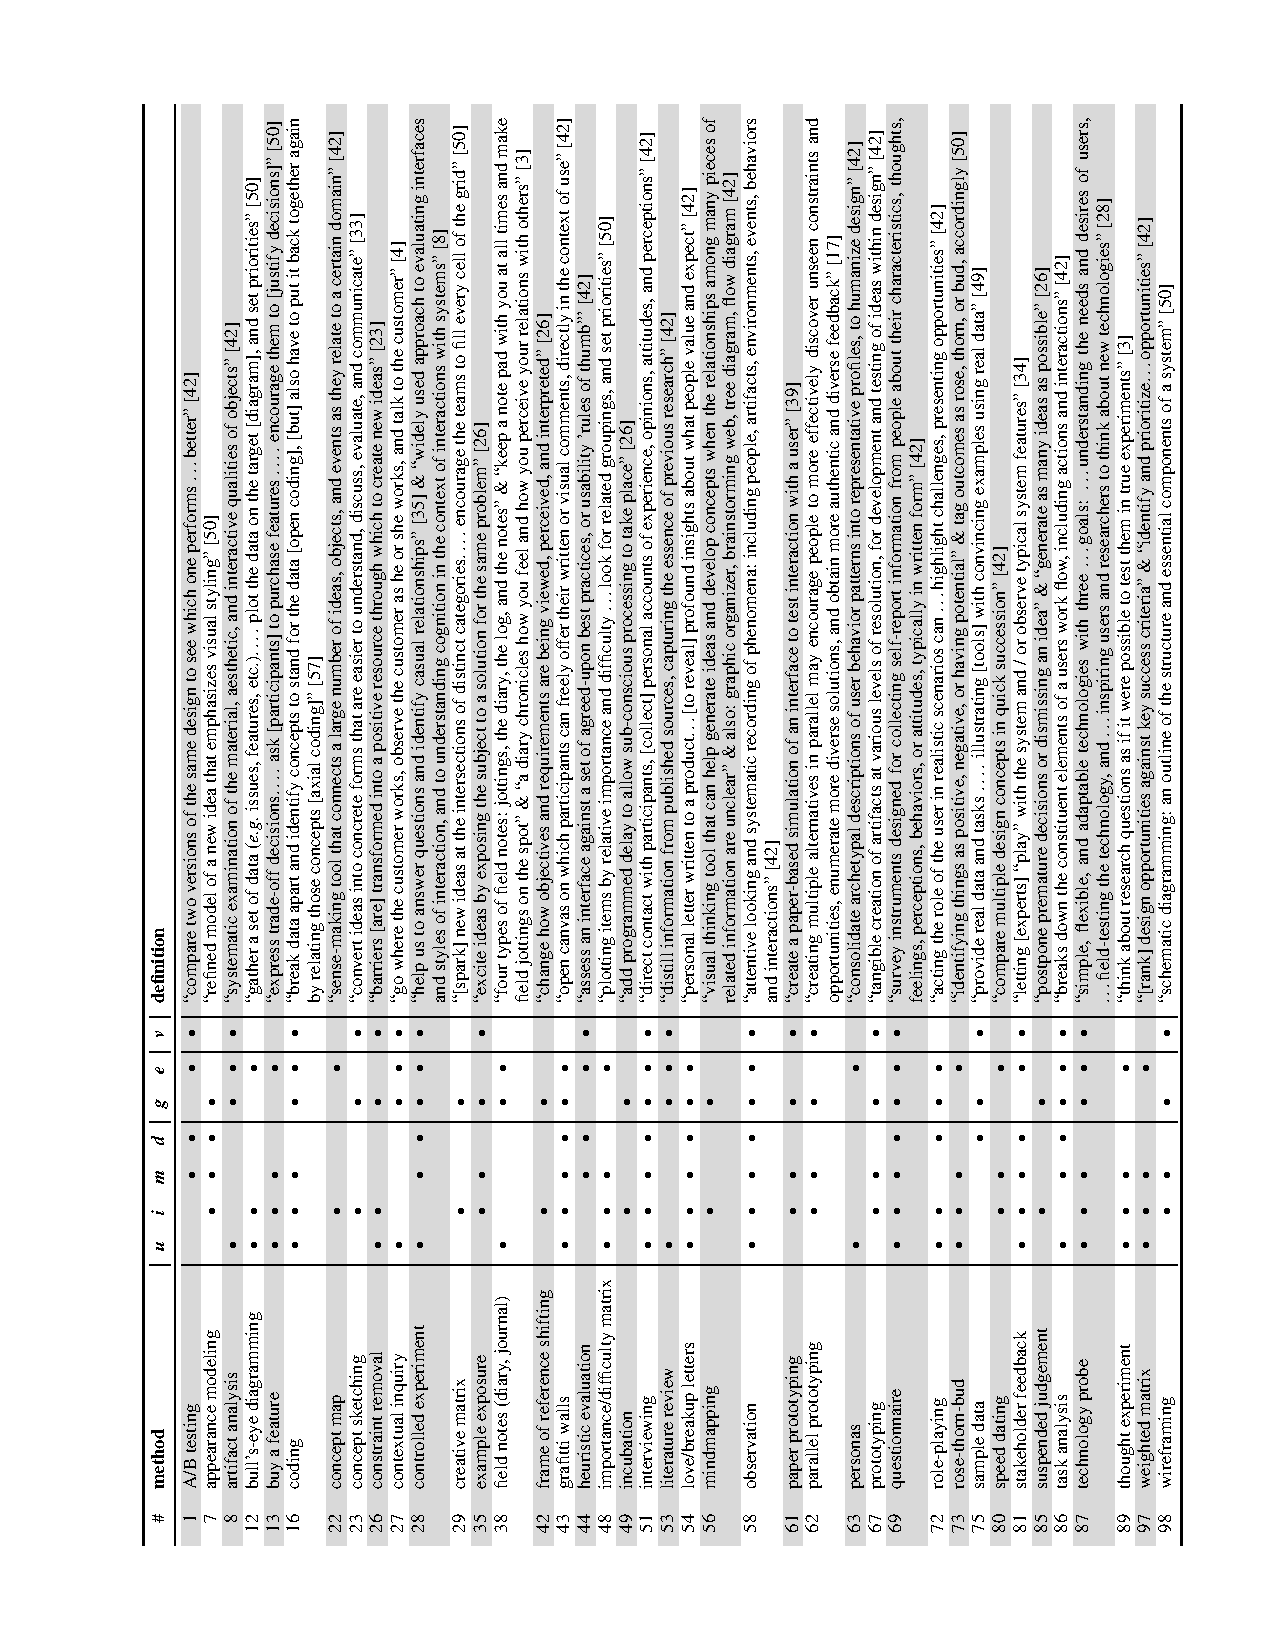
\includegraphics[width=1.00000\textwidth]{figures/daf/table.pdf}


% load table in on next page after reference
\afterpage{
\clearpage


% alternate row colors
\definecolor{light-gray}{gray}{0.85}
\rowcolors{1}{white}{light-gray}
\setlength\arrayrulewidth{1.0pt}


% methods table generated by Excel2LaTeX
\begin{sidewaystable*}[htbp]
\centering
\caption{
  Numerous exemplar methods and where they fit within the framework. A more
  extensive list of 100 methods is in Appendix~\ref{sec:app-methods}. We coded
  each method into one or more of the four design activities: \emph{understand}
  (\textbf{\emph{u}}), \emph{ideate} (\textbf{\emph{i}}), \emph{make}
  (\textbf{\emph{m}}), and \emph{deploy} (\textbf{\emph{d}}). Additionally, we
  tagged whether each method was largely generative (\textbf{\emph{g}}) or
  evaluative (\textbf{\emph{e}}), or both. Lastly, we categorized the methods we
  have seen commonly reported within the visualization community
  (\textbf{\emph{v}}) and also present succinct definitions for each method to
  assist designers in trying each method out.
}
\label{tbl:methods}
  \begin{tabular}{rl|cccc|cc|c|p{15cm}}
  \toprule
  \#    & \textbf{method} & \textit{\textbf{u}} & \textit{\textbf{i}} & \textit{\textbf{m}} & \textit{\textbf{d}} & \textit{\textbf{g}} & \textit{\textbf{e}} & \textit{\textbf{v}} & \textbf{definition} \\
  \midrule
  1     & A/B testing &       &       &  \sbt     &  \sbt     &       &  \sbt     &  \sbt     & ``compare two versions of the same design to see which one performs \ldots better'' \cite{Martin2012} \\
  7     & appearance modeling &       &  \sbt     &  \sbt     &  \sbt     &  \sbt     &       &       & ``refined model of a new idea that emphasizes visual styling'' \cite{Review2014} \\
  8     & artifact analysis &  \sbt     &       &       &       &  \sbt     &  \sbt     &  \sbt     & ``systematic examination of the material, aesthetic, and interactive qualities of objects'' \cite{Martin2012} \\
  12     & bull's-eye diagramming &  \sbt     &  \sbt     &       &       &       &  \sbt     &       & ``gather a set of data (e.g., issues, features, etc.)\ldots. plot the data on the target [diagram], and set priorities'' \cite{Review2014} \\
  13     & buy a feature &  \sbt     &  \sbt     &  \sbt     &       &       &  \sbt     &       & ``express trade-off decisions\ldots. ask [participants] to purchase features \ldots. encourage them to [justify decisions]'' \cite{Review2014} \\
  16     & coding &  \sbt     &  \sbt     &  \sbt     &       &  \sbt     &  \sbt     &  \sbt     & ``break data apart and identify concepts to stand for the data [open coding], [but] also have to put it back together again by relating those concepts [axial coding]'' \cite{Strauss1990} \\
  22     & concept map &       &  \sbt     &       &       &       &  \sbt     &       & ``sense-making tool that connects a large number of ideas, objects, and events as they relate to a certain domain'' \cite{Martin2012} \\
  23     & concept sketching &       &  \sbt     &       &       &  \sbt     &       &  \sbt     & ``convert ideas into concrete forms that are easier to understand, discuss, evaluate, and communicate'' \cite{Kumar2012} \\
  26     & constraint removal &  \sbt     &  \sbt     &       &       &  \sbt     &       &  \sbt     & ``barriers [are] transformed into a positive resource through which to create new ideas'' \cite{Goodwin2013a} \\
  27    & contextual inquiry &  \sbt     &       &       &       &  \sbt     &  \sbt     &  \sbt     & ``go where the customer works, observe the customer as he or she works, and talk to the customer'' \cite{Beyer1997} \\
  28    & controlled experiment &  \sbt     &       &  \sbt     &  \sbt     &  \sbt     &  \sbt     &  \sbt     & ``help us to answer questions and identify casual relationships'' \cite{Lazar2010} \& ``widely used approach to evaluating interfaces and styles of interaction, and to understanding cognition in the context of interactions with systems'' \cite{Cairns2008} \\
  29    & creative matrix &       &  \sbt     &       &       &  \sbt     &       &       & ``[spark] new ideas at the intersections of distinct categories\ldots. encourage the teams to fill every cell of the grid'' \cite{Review2014} \\
  35    & example exposure &       &  \sbt     &  \sbt     &       &  \sbt     &       &  \sbt     & ``excite ideas by exposing the subject to a solution for the same problem'' \cite{Hernandez2010} \\
  38    & field notes (diary, journal) &  \sbt     &       &       &       &  \sbt     &  \sbt     &       & ``four types of field notes: jottings, the diary, the log, and the notes'' \& ``keep a note pad with you at all times and make field jottings on the spot'' \& ``a diary chronicles how you feel and how you perceive your relations with others'' \cite{Bernard2011} \\
  42    & frame of reference shifting &       &  \sbt     &       &       &  \sbt     &       &       & ``change how objectives and requirements are being viewed, perceived, and interpreted'' \cite{Hernandez2010} \\
  43    & grafitti walls &  \sbt     &  \sbt     &  \sbt     &  \sbt     &  \sbt     &  \sbt     &       & ``open canvas on which participants can freely offer their written or visual comments, directly in the context of use'' \cite{Martin2012} \\
  44    & heuristic evaluation &       &       &  \sbt     &  \sbt     &       &  \sbt     &  \sbt     & ``assess an interface against a set of agreed-upon best practices, or usability 'rules of thumb''' \cite{Martin2012} \\
  48    & importance/difficulty matrix &  \sbt     &  \sbt     &  \sbt     &       &       &  \sbt     &       & ``plotting items by relative importance and difficulty \ldots look for related groupings, and set priorities'' \cite{Review2014} \\
  49    & incubation &       &  \sbt     &       &       &  \sbt     &       &       & ``add programmed delay to allow sub-conscious processing to take place'' \cite{Hernandez2010} \\
  51    & interviewing &  \sbt     &  \sbt     &  \sbt     &  \sbt     &  \sbt     &  \sbt     &  \sbt     & ``direct contact with participants, [collect] personal accounts of experience, opinions, attitudes, and perceptions'' \cite{Martin2012} \\
  53    & literature review &  \sbt     &       &       &       &  \sbt     &  \sbt     &  \sbt     & ``distill information from published sources, capturing the essence of previous research'' \cite{Martin2012} \\
  54    & love/breakup letters &  \sbt     &  \sbt     &  \sbt     &  \sbt     &  \sbt     &  \sbt     &       & ``personal letter written to a product\ldots [to reveal] profound insights about what people value and expect'' \cite{Martin2012} \\
  56    & mindmapping &       &  \sbt     &       &       &  \sbt     &       &       & ``visual thinking tool that can help generate ideas and develop concepts when the relationships among many pieces of related information are unclear'' \& also: graphic organizer, brainstorming web, tree diagram, flow diagram \cite{Martin2012} \\
  58    & observation &  \sbt     &  \sbt     &  \sbt     &  \sbt     &  \sbt     &  \sbt     &  \sbt     & ``attentive looking and systematic recording of phenomena: including people, artifacts, environments, events, behaviors and interactions'' \cite{Martin2012} \\
  61    & paper prototyping &       &  \sbt     &  \sbt     &       &  \sbt     &       &  \sbt     & ``create a paper-based simulation of an interface to test interaction with a user'' \cite{Maguire2001} \\
  62    & parallel prototyping &       &  \sbt     &  \sbt     &       &  \sbt     &       &  \sbt     & ``creating multiple alternatives in parallel may encourage people to more effectively discover unseen constraints and opportunities, enumerate more diverse solutions, and obtain more authentic and diverse feedback'' \cite{Dow2010} \\
  63    & personas &  \sbt     &       &       &       &       &  \sbt     &       & ``consolidate archetypal descriptions of user behavior patterns into representative profiles, to humanize design'' \cite{Martin2012} \\
  67    & prototyping &       &  \sbt     &  \sbt     &       &  \sbt     &       &  \sbt     & ``tangible creation of artifacts at various levels of resolution, for development and testing of ideas within design'' \cite{Martin2012} \\
  69    & questionnaire &  \sbt     &  \sbt     &  \sbt     &  \sbt     &  \sbt     &  \sbt     &  \sbt     & ``survey instruments designed for collecting self-report information from people about their characteristics, thoughts, feelings, perceptions, behaviors, or attitudes, typically in written form'' \cite{Martin2012} \\
  72    & role-playing &  \sbt     &  \sbt     &       &  \sbt     &  \sbt     &  \sbt     &       & ``acting the role of the user in realistic scenarios can \ldots highlight challenges, presenting opportunities'' \cite{Martin2012} \\
  73    & rose-thorn-bud &  \sbt     &  \sbt     &  \sbt     &       &       &  \sbt     &       & ``identifying things as positive, negative, or having potential'' \& tag outcomes as rose, thorn, or bud, accordingly \cite{Review2014} \\
  75    & sample data &       &       &       &  \sbt     &  \sbt     &       &  \sbt     & ``provide real data and tasks \ldots. illustrating [tools] with convincing examples using real data'' \cite{Plaisant2004} \\
  80    & speed dating &       &  \sbt     &  \sbt     &       &       &  \sbt     &       & ``compare multiple design concepts in quick succession'' \cite{Martin2012} \\
  81    & stakeholder feedback &  \sbt     &  \sbt     &  \sbt     &  \sbt     &       &  \sbt     &  \sbt     & ``letting [experts] ``play'' with the system and / or observe typical system features'' \cite{Lam2011a} \\
  85    & suspended judgement &       &  \sbt     &       &       &  \sbt     &       &       & ``postpone premature decisions or dismissing an idea'' \& ``generate as many ideas as possible'' \cite{Hernandez2010} \\
  86    & task analysis &  \sbt     &       &  \sbt     &  \sbt     &  \sbt     &  \sbt     &  \sbt     & ``breaks down the constituent elements of a user’s work flow, including actions and interactions'' \cite{Martin2012} \\
  87    & technology probe &  \sbt     &  \sbt     &  \sbt     &       &  \sbt     &  \sbt     &  \sbt     & ``simple, flexible, and adaptable technologies with three \ldots goals: \ldots  understanding the needs and desires of users, \ldots field-testing the technology, and \ldots inspiring users and researchers to think about new technologies'' \cite{Hutchinson2003a} \\
  89    & thought experiment &  \sbt     &  \sbt     &  \sbt     &       &       &  \sbt     &       & ``think about research questions as if it were possible to test them in true experiments'' \cite{Bernard2011} \\
  97    & weighted matrix &  \sbt     &  \sbt     &  \sbt     &       &       &  \sbt     &       & ``[rank] design opportunities against key success criteria'' \& ``identify and prioritize\ldots opportunities'' \cite{Martin2012} \\
  98    & wireframing &       &  \sbt     &  \sbt     &       &  \sbt     &       &  \sbt     & ``schematic diagramming: an outline of the structure and essential components of a system'' \cite{Review2014} \\
  \bottomrule
  \end{tabular}
\end{sidewaystable*}
\newpage
}
